\section{The experiments under calibrated noise}
\label{sec:noise}

\subsection{Seven machines as noise models}
\label{sec:devices}

For each of seven quantum computers we collected the vendor's published calibration numbers
--- two-qubit and one-qubit gate error, gate durations, $T_1$, $T_2$, readout error, and the
qubit connectivity --- into a device file whose every field carries the URL it was read from,
the retrieval date (20 August 2026) and a verbatim quotation (\cref{app:provenance}).
\Cref{tab:devices} summarises them.  Three things are worth knowing before reading any noise
result.  \emph{Quantinuum publishes no gate durations and no $T_1$/$T_2$}; its idle error is
instead charged from its published ``memory error per depth-1 circuit time''
($2.0\times10^{-4}$ for H2-1, $2.2\times10^{-4}$ for H1-1), and its simulated noise contains
no idle error at all.  \emph{Rigetti publishes only a two-qubit error} for Ankaa-3 (and the
99.5\,\% headline is for a different gate than the universal one we need); every Rigetti number
below is therefore an upper bound on the machine.  \emph{IQM's $T_1$/$T_2$ are a third-party
snapshot}, not vendor data, and its $T_2$ measured without echo is $8.5$\,µs against the
$21$\,µs echo value we use.  Where a vendor publishes no number we model that channel as
error-free and say so, rather than invent one.

\begin{table}[t]
\centering\small
\caption{The seven device presets (medians where the vendor publishes per-qubit tables).
Two-qubit error $\varepsilon_2$, one-qubit error $\varepsilon_1$, readout error (mean of
$p_{01}$, $p_{10}$), coherence times, two-qubit gate time.  ``—'' = not published; the
provenance of every entry is in \cref{app:provenance}.}
\label{tab:devices}
\begin{tabular}{@{}l l S[table-format=1.2e-1] S[table-format=1.1e-1] S[table-format=1.1e-1] l l S[table-format=5.0]@{}}
\toprule
Machine & Connectivity & {$\varepsilon_2$} & {$\varepsilon_1$} & {readout} & $T_1$ & $T_2$ & {2q gate (ns)} \\
\midrule
Quantinuum H1-1 & all-to-all & 9.7e-4 & 1.8e-5 & 2.3e-3 & — & — & {—} \\
Quantinuum H2-1 & all-to-all & 1.1e-3 & 1.9e-5 & 1.0e-3 & — & — & {—} \\
IonQ Forte & all-to-all & 4.0e-3 & 2.0e-4 & 5.0e-3 & 55\,s & 1\,s & 950000 \\
Google Willow & square & 4.1e-3 & 5.3e-4 & 8.0e-3 & 68\,µs & 89\,µs & 42 \\
IBM Fez (Heron r2) & heavy-hex & 3.9e-3 & 2.3e-4 & 7.7e-3 & 145\,µs & 88\,µs & 84 \\
IQM Garnet & square & 4.9e-3 & 8.0e-4 & 3.0e-2 & 27\,µs & 21\,µs & 30 \\
Rigetti Ankaa-3 & square & 1.0e-2 & {—} & {—} & — & — & 72 \\
\bottomrule
\end{tabular}
\end{table}

\subsection{Bit-count}
\label{sec:noise-bitcount}

The trained 11-qubit bit-count networks (prototype and classic) were evaluated exactly, as
density matrices on the GPU, under each preset
(run \run{bitcount\_noise/20260820T145335Z}; \cref{fig:bitcount-noise-devices}).  The model
distribution moves by a total-variation distance of $0.005$ (Quantinuum H2-1) to $0.039$ (IQM
Garnet); the KL to the target rises from $5.5\times10^{-4}$ to $7\times10^{-4}$ on H2-1 and to
$6\times10^{-3}$ on Garnet.  The prototype network is better than the classic one under every
preset, but the displacement \emph{caused} by the noise ($\KL(\text{clean}\,\|\,\text{noisy})$,
median $0.0021$ vs $0.0022$) is the same for both: both have identical two-qubit gate counts,
and the prototype's advantage under noise is inherited from its better noiseless fit, not from
any robustness of the neuron type.  Scaling IBM Fez's noise by $s$
(\cref{fig:bitcount-noise-scale}) gives $\KL\propto s^{1.7}$ and $\TV\propto s^{0.95}$ --- a
linear response.

Can one train \emph{under} the noise?  On a 7-qubit version of the network (3 inputs, 3 hidden;
the 11-qubit grid would have cost 13 hours and was not run) the answer is yes
(\cref{fig:bitcount-noise-aware}): training with the noise model in the loop recovers the noisy
KL by a median factor of $158$ (prototype) and $361$ (classic) --- but the recovered parameters
are \emph{worse} on a noiseless simulator, i.e.\ the optimiser folds the channel into the
angles rather than finding noise-robust ones.

\begin{figure}[t]
\centering
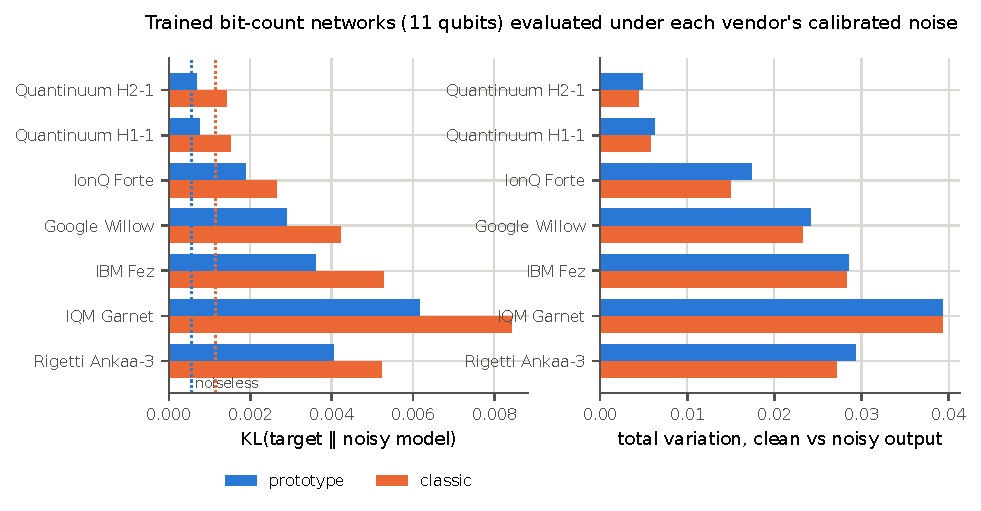
\includegraphics[width=\textwidth]{fig_bitcount_noise_devices}
\caption{The trained bit-count networks under each machine's noise model.  Left: KL to the
target (dotted lines: the noiseless values).  Right: how far the output distribution moved.
Rigetti's row models only its two-qubit error.  Run \run{bitcount\_noise/20260820T145335Z}.}
\label{fig:bitcount-noise-devices}
\end{figure}

\begin{figure}[t]
\centering
\begin{minipage}[t]{0.5\textwidth}\centering
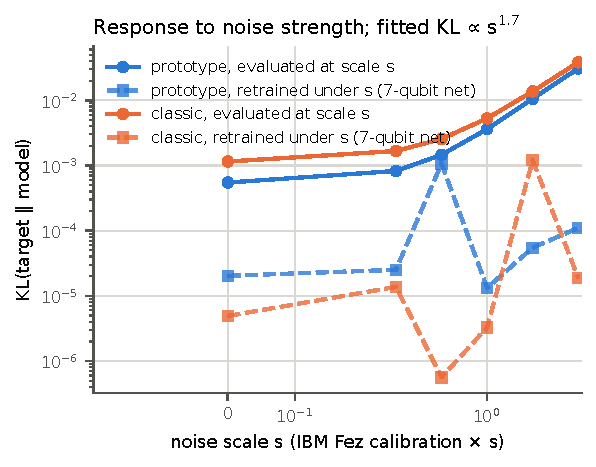
\includegraphics[width=\textwidth]{fig_bitcount_noise_scale}
\caption{Response to noise strength: IBM Fez's calibration scaled by $s$ (solid), and a
7-qubit network retrained with the scaled noise in the loop (dashed).  Same run.}
\label{fig:bitcount-noise-scale}
\end{minipage}\hfill
\begin{minipage}[t]{0.47\textwidth}\centering
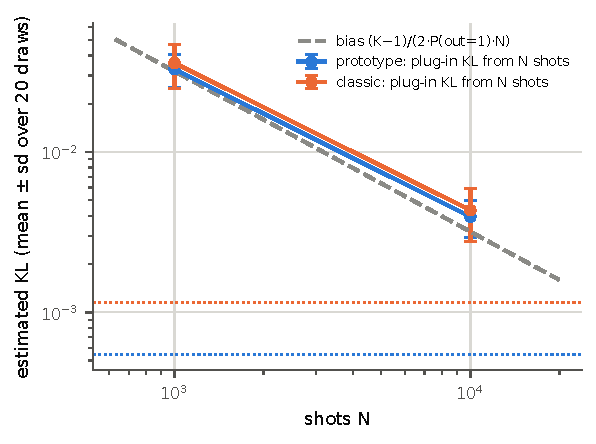
\includegraphics[width=\textwidth]{fig_bitcount_plugin_bias}
\caption{Estimating the KL from $N$ shots: the plug-in estimate sits above the true value by
$(K-1)/(2\,\Pout\,N)$, with $K=32$ bins and only $\Pout\approx 0.49$ of the shots usable.}
\label{fig:plugin-bias}
\end{minipage}
\end{figure}

\begin{figure}[t]
\centering
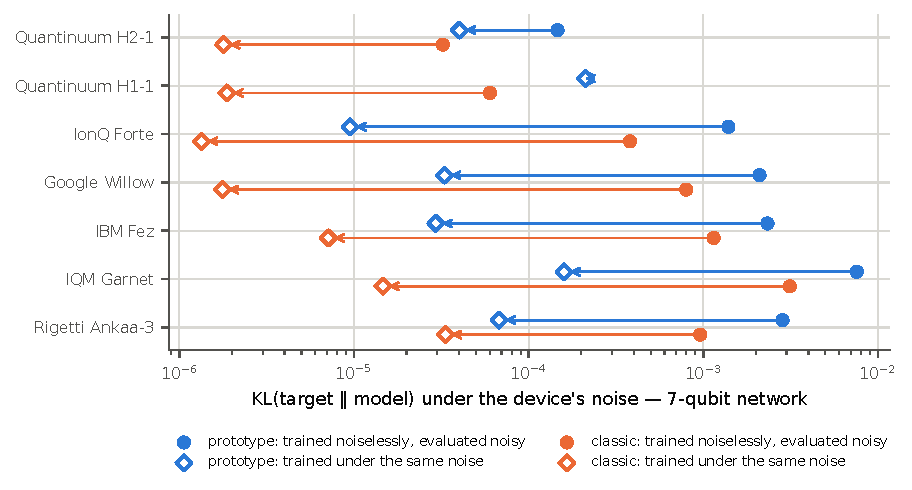
\includegraphics[width=0.9\textwidth]{fig_bitcount_noise_aware}
\caption{Noise-aware training (7-qubit bit-count network, three seeds): KL under each
machine's noise for parameters trained noiselessly (filled) and for parameters trained with the
same noise model in the loop (open), median of three seeds.}
\label{fig:bitcount-noise-aware}
\end{figure}

\subsection{Flappy Bird}
\label{sec:noise-flappy}

The Flappy controller is a thresholded activation, so what matters is not how far $\Pout$ moves
but whether it crosses $\tfrac12$.  Evaluated exactly under every preset on its $65\times65$
decision grid and then played for 20 held-out games (run
\run{flappy\_noise/20260820T154249Z}; \cref{fig:flappy-noise}, left), the controller \emph{still
plays perfectly on all seven machines}: only $1.5$--$4\,\%$ of the frames it actually visits are
decided differently, because the noise contracts every activation toward $\tfrac12$ by about the
same amount (mean $|\Delta P| = 0.002$--$0.018$) and so rarely changes the ordering
$P\gtrless\tfrac12$.  There is a factor of two of headroom: IBM Fez's noise scaled by $2$ leaves
$60\,\%$ of games perfect, by $4$ none (\cref{fig:flappy-noise}, right).

Shot noise is a different matter (\cref{fig:flappy-shot-noise}).  Re-deciding every frame from
$N$ measurements of the output qubit, the same controller wins no game at $N=1\,000$, $90\,\%$
at $4\,000$ and all at $10\,000$ on a noiseless simulator; on IBM Fez's model only $55\,\%$ at
$4\,000$.  The reason is the distribution of decision margins over the frames the agent plays:
median $\delta = 0.019$, tenth percentile $0.004$, first percentile $0.0002$ (right panel).  The
measured flip rate per frame agrees with the average of $\Phi(-2\delta\sqrt N)$ over that
distribution to $3\,\%$.  A deterministic shift of the boundary (gate noise) is tolerated far
past a stochastic one: Fez at scale $2$ decides $20\,\%$ of frames differently and still wins
$60\,\%$ of games; $1\,000$ shots decide only $8.5\,\%$ differently and win none.  A controller
that is re-rolled every frame is a jittery controller, and two or three unlucky frames in a row
are a collision.  Fine-tuning under Fez's noise for five sweeps changes nothing (the training
episodes already all survive, so the objective has no slope).

\begin{figure}[t]
\centering
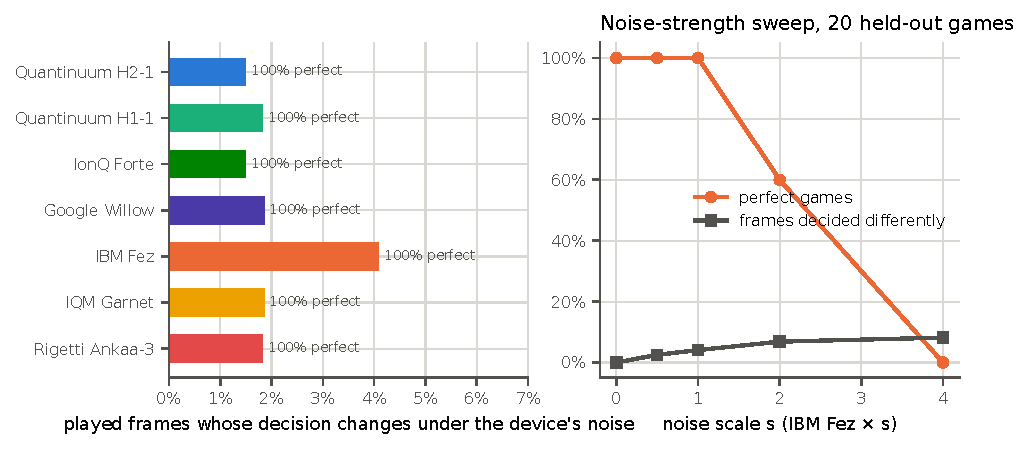
\includegraphics[width=\textwidth]{fig_flappy_noise}
\caption{Flappy under gate noise.  Left: fraction of played frames whose decision changes
under each machine's model; every machine still yields $100\,\%$ perfect games.  Right: IBM
Fez's noise scaled by $s$.  Run \run{flappy\_noise/20260820T154249Z}.}
\label{fig:flappy-noise}
\end{figure}

\begin{figure}[t]
\centering
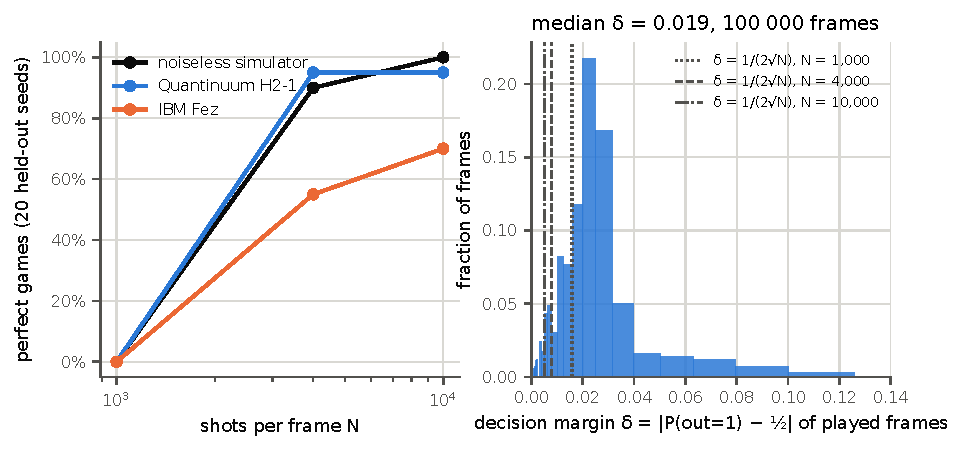
\includegraphics[width=\textwidth]{fig_flappy_shot_noise}
\caption{Flappy under shot noise.  Left: perfect games when every frame is decided from $N$
shots.  Right: distribution of the decision margin $\delta$ over the $100\,000$ frames the
noiseless controller plays; the vertical lines mark the margin that $N$ shots can just resolve.
Same run.}
\label{fig:flappy-shot-noise}
\end{figure}

\subsection{ECG and Iris (reduced run)}
\label{sec:noise-ecg-iris}

The ECG and Iris grids were run in a \emph{reduced} configuration only (run
\run{ecg\_iris\_noise/20260820T155618Z}): ECG on 8 test windows instead of 898 and two presets
instead of seven; Iris with 16 Monte-Carlo trajectories per evaluation instead of 2\,000 (per-outcome
standard error $\approx 12\,\%$), two presets, and perfect preparation of the dataset state
assumed.  The measured cost of the full grids --- 4--6 CPU-hours for ECG, 8 hours for Iris --- put
them outside the session's budget, and they were not run.  What the reduced run shows
(\cref{fig:ecg-iris-noise}) is indicative only: ECG denoising loses $-0.1$ to $+0.4$~dB under
Quantinuum H2-1 and $1.6$--$2.7$~dB (classic) under IBM Fez, while the prototype cells
\emph{gain} up to $3.8$~dB under Fez on eight windows --- a small-sample artefact, not a finding.
Iris keeps its $95\,\%$ accuracy under H2-1 and loses it under Fez ($64\pm44\,\%$ over two
trajectory seeds) for the prototype network, whose read-out is a conditional distribution over
4\,096 input strings and therefore directly exposed to probability leaking out of the 20-code
support.  One noisy sweep of ECG fine-tuning gains $2.7$~dB under Fez and $3.7$~dB noiselessly
--- it finishes the clean optimisation, it does not fold the channel in.

\begin{figure}[t]
\centering
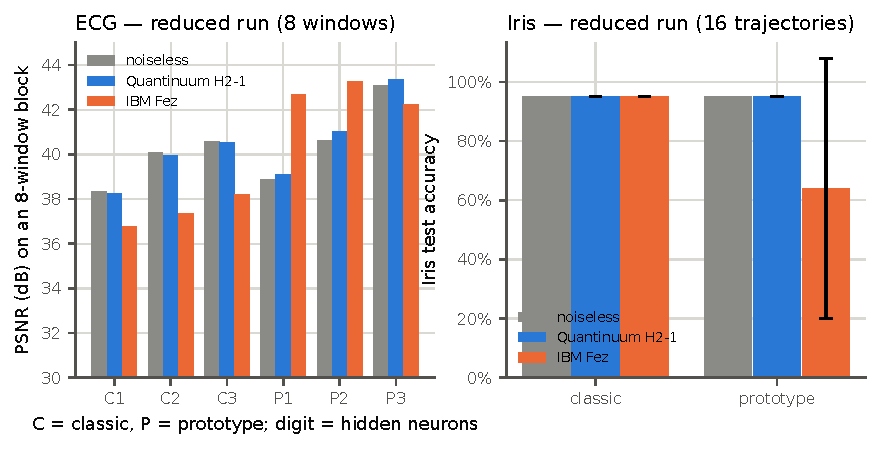
\includegraphics[width=\textwidth]{fig_ecg_iris_noise}
\caption{Reduced-configuration noise runs, quoted for the record.  Left: ECG PSNR on an
8-window block.  Right: Iris test accuracy from 16 trajectories (error bars: two trajectory
seeds).  Run \run{ecg\_iris\_noise/20260820T155618Z}.}
\label{fig:ecg-iris-noise}
\end{figure}
